
\begin{figure}[htb]
  % Requires \usepackage{graphicx}
  \centering
  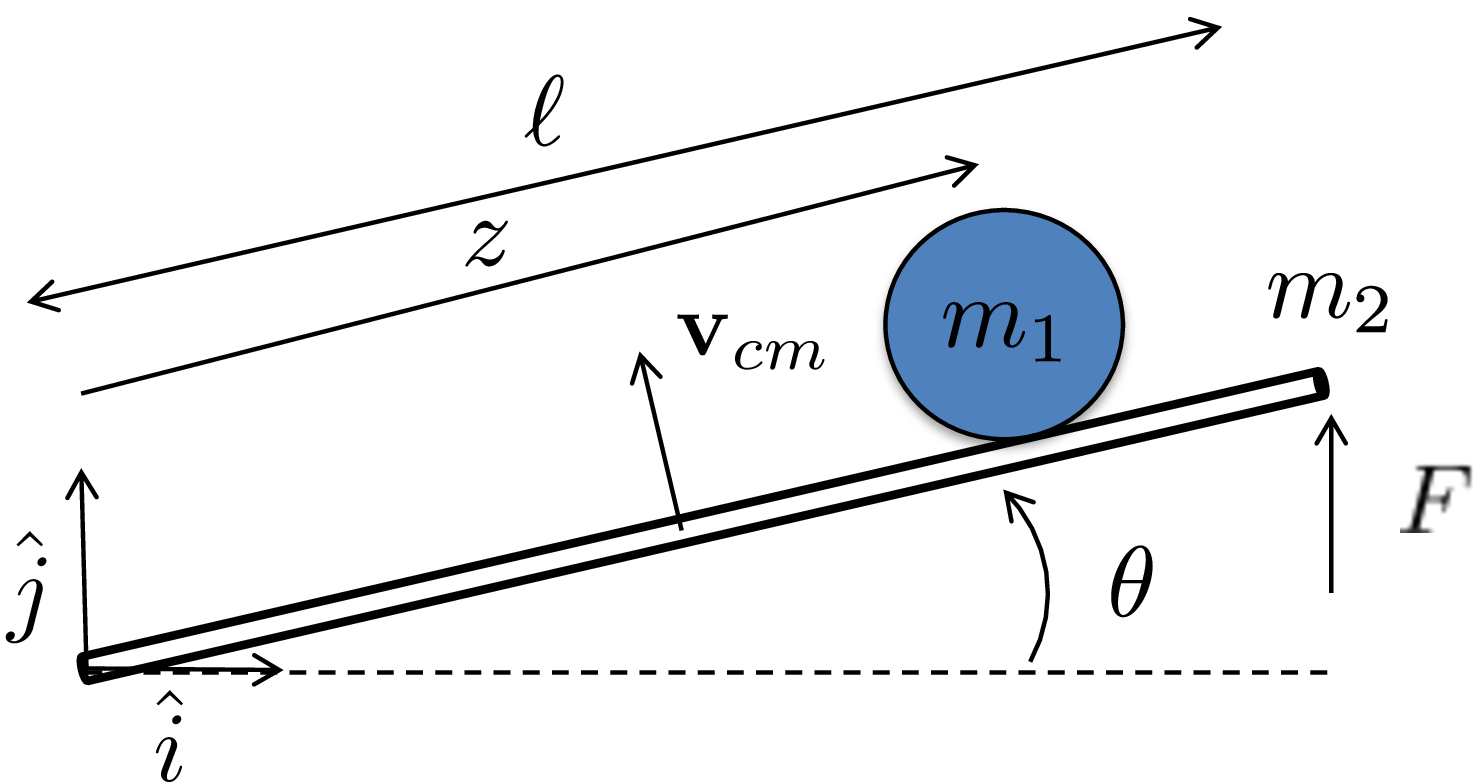
\includegraphics[width=0.8\textwidth]{6_design_studies/figures/hw_ballbeam_kinetic_energy}
  \caption{Finding the kinetic energy for the ball on beam system.}
  \label{fig:hw_ballbeam_kinetic energy}
\end{figure}

The generalized coordinates for the system are the position of the ball along the beam $z$ and the angle of the beam $\theta$.  Therefore, let $\mathbf{q} = (z, \theta)^\top$.

Let $P_0$ be the potential energy when $z=0$ and $\theta=0$.  Then the potential energy of the ball on beam system is the sum of the potential energy of the center of mass of the beam, and the potential energy of the ball, modeled as a point mass:
\begin{equation*}
  P = P_0 + m_1 g z \sin\theta + \frac{m_2 g l}{2} \sin\theta.
\end{equation*}

The external forces acting in the direction of $z$ is $\tau_1 = 0$, and the external torque acting in the direction of $\theta$ is $\tau_2= F \ell\cos\theta$.  Therefore, the generalized forces are $\boldsymbol{\tau}=(0, F\ell\cos\theta)^\top$.  We will assume that the ball rolls without friction and that there is no friction in the pivot point.  Therefore, there is no damping in the system.

From problem \ref{hw:ballbeam}.1, the kinetic energy can be written in terms of the generalized coordinates as
\begin{align*}
K(\mathbf{q},\dot{\mathbf{q}}) &=   \frac{1}{2} m_1 \dot{z}^2 + \frac{1}{2} \left( \frac{m_2 \ell^2 }{3} + m_1 z^2 \right) \dot{\theta}^2
 \\
&= \frac{1}{2} m_1 \dot{q}_1^2 + \frac{1}{2} \left( \frac{m_2 \ell^2 }{3} + m_1 q_1^2 \right) \dot{q}_2^2,
\end{align*}
and the potential energy can be written as
\begin{align*}
P(\mathbf{q}) &= P_0 + m_1 g q_1 \sin q_2 + \frac{m_2 g l}{2} \sin q_2.
\end{align*}
The Lagrangian is therefore given by
\[
L(\mathbf{q},\dot{\mathbf{q}}) = \frac{1}{2} m_1 \dot{z}^2 + \frac{1}{2} \left( \frac{m_2 l^2 }{3} + m_1 z^2 \right) \dot{\theta}^2 - P_0 - m_1 g z \sin(\theta) - \frac{m_2 g l}{2} \sin(\theta).
\]
The Euler Lagrange equations are
\begin{align*}
\frac{d}{dt} \left( \frac{\partial L}{\partial \dot{z}} \right) - \frac{\partial L}{\partial z} &= \tau_1 \\
\frac{d}{dt} \left( \frac{\partial L}{\partial \dot{\theta}} \right) - \frac{\partial L}{\partial \theta} &= \tau_2,
\end{align*}
where
\begin{align*}
\frac{\partial L}{\partial \dot{z}} &= m_1 \dot{z} \\
\frac{d}{dt} \left( \frac{\partial L}{\partial \dot{z}} \right) &= m_1 \ddot{z} \\
\frac{\partial L}{\partial z} &= m_1 z \dot{\theta}^2 - m_1 g \sin{\theta} \\
\frac{\partial L}{\partial \dot{\theta}} &= \left( \frac{m_2 \ell^2 }{3} + m_1 z^2 \right) \dot{\theta} \\
\frac{d}{dt} \left( \frac{\partial L}{\partial \dot{\theta}} \right) &= \left( \frac{m_2 \ell^2}{3} + m_1 z^2 \right) \ddot{\theta} + 2 m_1 z \dot{z} \dot{\theta} \\
\frac{\partial L}{\partial \theta} &= - m_1 g z \cos(\theta) - \frac{m_2 g \ell}{2} \cos(\theta).
\end{align*}

Therefore the equations of motion are
\begin{align*}
 m_1\ddot{z} - m_1 z \dot{\theta}^2 + m_1 g \sin\theta &= 0 \\
\left( \frac{m_2 \ell^2}{3} + m_1 z^2 \right) \ddot{\theta} + 2 m_1 z \dot{z} \dot{\theta} + m_1 g z \cos{\theta} + \frac{m_2 g \ell}{2} \cos{\theta} &= F \ell \cos{\theta}.
\end{align*}

Using matrix notation, this equation can be rearranged to isolate the second order derivatives on the left and side
\begin{equation}\label{eq:ballbeam_sim_model}
\begin{pmatrix}
m_1 & 0  \\ 
0 & \left( \frac{m_2 \ell^2}{3} + m_1 z^2 \right)
\end{pmatrix} 
	\begin{pmatrix}\ddot{z} \\ \ddot{\theta} \end{pmatrix}
= \begin{pmatrix}   m_1 z \dot{\theta}^2 - m_1 g \sin\theta \\ F \ell \cos\theta - 2 m_1 z \dot{z} \dot{\theta} - m_1 g z \cos\theta 
	- \frac{m_2 g \ell}{2} \cos\theta \end{pmatrix}.
\end{equation}
Equation~\eqref{eq:ballbeam_sim_model} represents the simulation model for the ball on beam system.





